\section{Peer Unit}
\label{sec:peer}

\emph{Peer} unit is an input source that  sends BGP messages over the BGP peering session. \emph{Peer} unit includes \emph{IPv4 Peer} and \emph{IPv6 Peer} setups that are necessary for testing IPv4 and IPv6 peering function in BGPmon test instance. Overall, \emph{Peer} unit has following goals:

\begin{itemize}
\item{Keep BGP session: its important to verify that BGPmon can keep peering session alive with  IPv4 or IPv6 enabled peer.}
\item{Receive routes: this verifies that BGPmon is able to receive BGP update messages from IPv4 or IPv6 peer.}
\item{Test BGP capabilities: this verifies that BGPmon is able to work with any BGP capabilities.}
\end{itemize}



\subsection{IPv4 Peer Unit Overview}

\begin{figure}
\centering
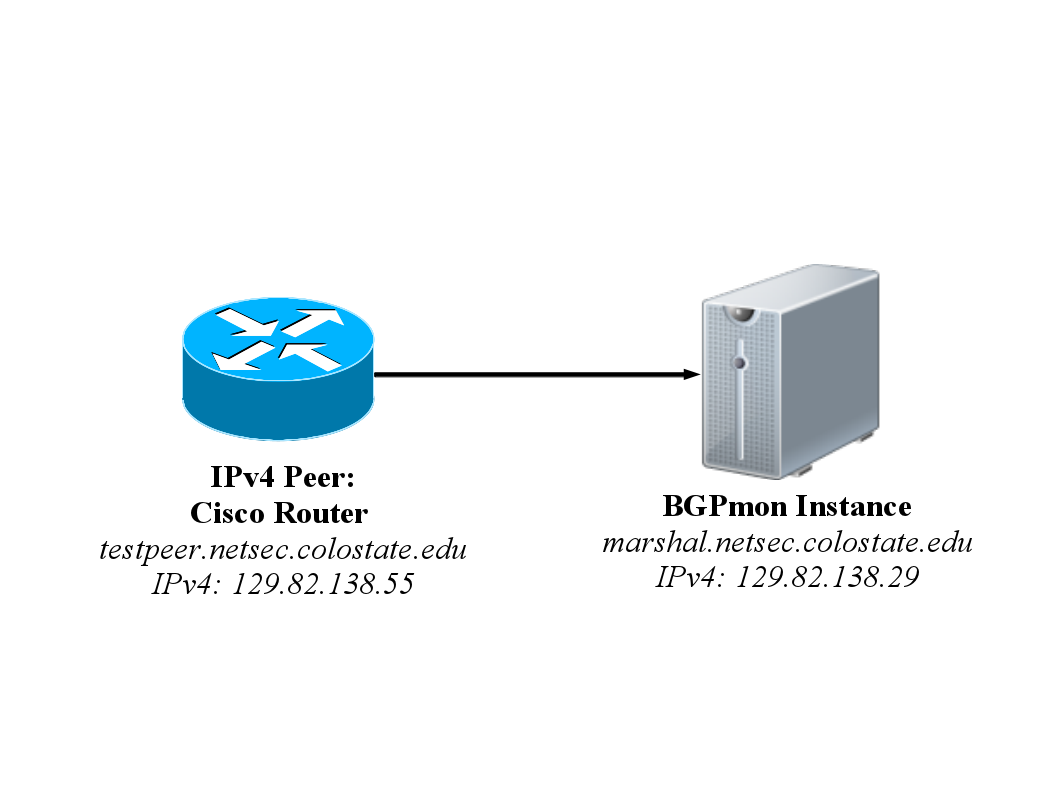
\includegraphics[scale=0.30]{figs/ipv4-peer.png}
\caption{An overview of IPv4 Peering Unit.}
\label{peerv4}
\end{figure}

Figure \ref{peerv4} shows a test unit design: it has IPv4-enabled Cisco router and testing instance of BGPmon.   Cisco router is configured on \emph{testpeer.netsec.colostate.edu} with \emph{129.82.138.55} IPv4 address.  BGPmon test instance is installed on \emph{marshal.netsec.colostate.edu} with \emph{129.82.138.29} IPv4 address.    In order to run \emph{IPv4 Peer} unit, user of the framework need to be familiar with Cisco router default configuration and BGPmon default configuration that is used for BGP peering session.

\subsubsection{IPv4 Peer Unit Launch}

To launch BGP peering session between Cisco router and BGPmon test instance:
\begin{enumerate}
\item{Power on Cisco router in NetSec server room. This will enable Cisco \emph{default configuration}. \emph{Default configuration} setup is discussed in details in  Section \ref{sec:ipv4ciscodef}.}
\item{Login to \emph{marshal.netsec.colostate.edu}}
  \begin{enumerate}
  \item{Make sure that BGPmon process is up and running. If not, see Section \ref{sec:essentials}.}
  \item{Telnet to \emph{localhost} port \emph{50000} to Command Line Interface.}
  \item{In \emph{router mode}, launch:}
    \begin{verbatim}
marshal(config)# neighbor 129.82.138.55 enable
    \end{verbatim}
   \item{This configuration enabled BGP peer session between BGPmon and Cisco router.} 
  \end{enumerate}
\end{enumerate}

There are few important tips that user of framework need to know while running the \emph{IPv4 Peer} unit. 

\begin{enumerate}

\item{For testing BGP capabilities, BGP peering session may need restart.  To reload peer settings and restart peer session, run following in Cisco's telnet:}
\begin{verbatim}
testpeer#clear ip bgp 129.82.138.29
\end{verbatim}

\item{ User of framework may reload \emph{default configuration} at any time. This may be useful in starting the new test or in case having misconfiguration in Cisco router. In order to restart \emph{default configuration}, run:}
\begin{verbatim}
testpeer#reload
System configuration has been modified. Save? [yes/no]: no
Proceed with reload? [confirm]
\end{verbatim}

\item{User may want to configure Cisco router to announce another network prefix. Cisco router announce network prefixes that it can reach. For example, to start announcing \emph{11.0.0.0/8} prefix, Cisco router need to be able to reach this prefix via one of interfaces. Thus, full reconfiguration of network interfaces is required. See Section \ref{sec:ipv4ciscodef} for setting up \emph{default configuration}}. 

\end{enumerate}

\subsubsection{Cisco Router Default Configuration}
\label{sec:ipv4ciscodef}

Cisco router has minimal set of settings to create BGP session with BGPmon test instance.  This section describes Cisco's \emph{default state} and IOS configuration that enables this state. Any configuration requires telnet access to Cisco router. 

Figure \ref{peerv4} shows Cisco instance that has \emph{testpeer.netsec.colostate.edu} hostname. To configure hostname, run following command in \emph{configure mode}:
\begin{verbatim}
testpeer(config)#hostname testpeer.netsec.colostate.edu
\end{verbatim}

In order to configure BGP peering settings, Cisco router requires configuration of two network interfaces.  First network interface is configured to \emph{129.82.138.0/23} subnet and has \emph{129.82.138.55} IPv4 address. \emph{129.82.138.0/23} network is a network of NetSec Group at Colorado State University and \emph{129.82.138.55} IP address should be used for Cisco router only.   Second network interface is setup of \emph{139.179.0.0/16} subnet with \emph{139.179.96.1} IPv4 address. \emph{139.179.0.0/16} subnet is used for test purpose only and it should never appear in global routing table or anywhere else except the Test Framework. 

To configure first network interface, run following command in Cisco's telnet:
\begin{verbatim}
testpeer(config)#interface FastEthernet 0/0 
testpeer(config-if)#ip address 129.82.138.55 255.255.255.128
testpeer(config-if)#no shutdown
\end{verbatim}

To configure second network interface, run:
\begin{verbatim}
testpeer(config)#interface FastEthernet 1/0 
testpeer(config-if)#ip address 139.179.96.1 255.255.0.0
testpeer(config-if)#no shutdown
\end{verbatim}

In Figure \ref{peerv4} Cisco router and BGPmon instance negotiate peering session.  Cisco router uses following network configuration for peering: 
\begin{itemize}
  \item{IPv4 address: \emph{129.82.138.55}.}
  \item{AS number: \emph{64513}.}
\end{itemize}

To bring up BGP peering session, user need to enable IP routing and configure network prefix. Run following in telnet:

\begin{verbatim}
testpeer(config)#router bgp 64515
testpeer(config)#network 139.179.0.0 255.255.0.0
\end{verbatim}

To enable BGP peering session with BGPmon test instance, run:

\begin{verbatim}
testpeer(config)#neighbor 129.82.138.55 remote-as 64515 
testpeer(config)#end
\end{verbatim}

Installation above is  minimal set of configuration rules that \emph{IPv4 Peer} unit require.

In order to have this state permanently,  user need to save this configuration as  \emph{default configuration}.  To save, run following command:

\begin{verbatim}
testpeer#copy running-config startup-config
\end{verbatim}

This command saves Cisco \emph{default configuration} to the startup configuration file in NVRAM. \emph{Default configuration} set is used everytime when Cisco router is turned on.


\subsubsection{BGPmon Test Instance Default Configuration}
\label{sec:bgpmondef}

By default BGPmon application is installed on \emph{marshal.netsec.colostate.edu} and uses \emph{129.82.138.29} IPv4 address and \emph{64515} AS number for BGP peering session with Cisco router. 

To enable BGP peering session, run following command in \emph{router mode} in CLI:
\begin{verbatim}
marshal(config)# neighbor 129.82.138.55 enable
\end{verbatim}


\subsubsection{Result Reporting}

In order to verify if peering configuration in BGPmon was successfully enabled, run following command in \emph{privileged mode} in CLI of BGPmon test instance:
\begin{verbatim}
marshal#show bgp neighbor 129.82.138.55
\end{verbatim}

This command shows status information about peering session, both BGPmon and Cisco configuration values,  announced BGP capabilities and others.

In order to check that BGPmon received BGP update message from Cisco router, run following command:
\begin{verbatim}
marshal# show bgp routes 129.82.138.55
\end{verbatim}

This command shows IPv4 prefix that Cisco router announce. Also, it includes NextHop, AS path, AS length information from Cisco peer. 

In order to verify if peering configuration in Cisco router was enabled,  Cisco router provides a report of IPv4 peering session with BGPmon. To verify that IPv4 peering session is established and running,  run following in \emph{configuration mode} in Cisco's telnet:  

\begin{verbatim}
marshal# show ip bgp neighbors 129.82.138.29
\end{verbatim}

This command will show the status of IPv4 peering on Cisco router.  For example, in case of successfully configured peering session it will show following log:

\begin{verbatim}
BGP neighbor is 129.82.138.29,  remote AS 64515, external link
BGP version 4, remote router ID 129.82.138.29
BGP state = Established
\end{verbatim}




\subsection{IPv6 Peer Unit}

\begin{figure}
\centering
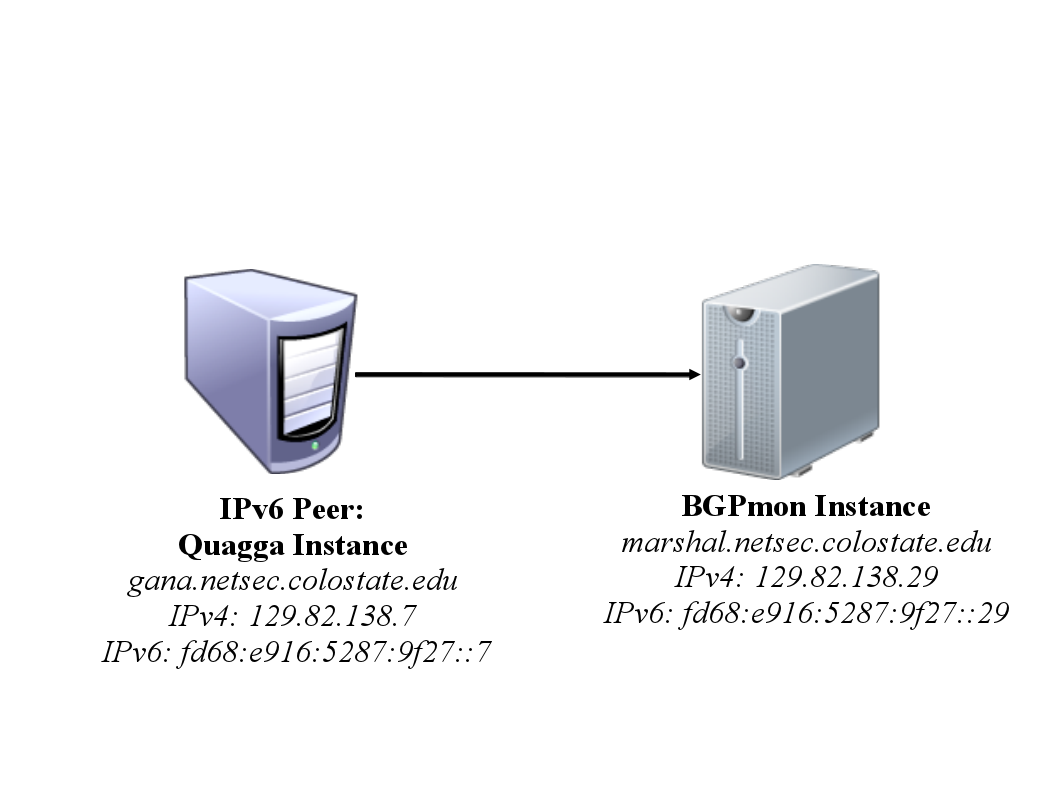
\includegraphics[scale=0.30]{figs/ipv6-peer.png}
\caption{An overview of IPv4 Peering Unit.}
\label{peerv6}
\end{figure}


\emph{IPv6 Peer} unit includes setup of Quagga Routing Suite software and BGPmon instance.     Due to the old version of Cisco IOS in \emph{IPv4 Peer} unit and lack of IPv6 protocol support in IOS,   Quagga  Routing Suite software was choosen to run BGP peering session with BGPmon instance.  Figure \ref{peerv6} shows a \emph{IPv6 Peer} unit design: it has dual-stack IPv4 and IPv6 enabled Quagga and BGPmon instances.   Quagga instance is installed on  \emph{gana.netsec.colostate.edu} and it has one physical network interface that configured for IPv4 and IPv6 IP addresses.   Quagga instance has following  configuration for BGP peering session with BGPmon test instance:
\begin{itemize}
  \item{Hostname: \emph{gana.netsec.colostate.edu}}
  \item{IPv4 address: \emph{129.82.138.7}}
  \item{IPv6 address: \emph{fd68:e916:5287:9f27::7}}
  \item{AS number: \emph{64514}}
\end{itemize}

BGPmon is installed on \emph{marshal.netsec.colostate.edu} with IPv4 and IPv6 addresses. BGPmon test instance use following configuration for BGP peering session with Quagga: 
\begin{itemize} 
  \item{Hostname: \emph{marshal.netsec.colostate.edu}.}
  \item{IPv4 address: \emph{129.82.138.29}.}
  \item{IPv6 address: \emph{fd68:e916:5287:9f27::29}.}
  \item{AS number: \emph{64515}.}
\end{itemize}

In order to run \emph{IPv46Peer} unit, user of the framework need to be familiar with Quagga and BGPmon configurations that are used for BGP peering over IPv6 protocol.

\subsubsection{IPv6 Peer Unit Launch}

To launch BGP peering session between Quagga instance and BGPmon test instance:




\begin{enumerate}
\item{Login to \emph{gana.netsec.colostate.edu}}
  \begin{enumerate}
    \item{Make sure that \emph{bgpd} processes is up and running. {Bgpd} process uses \emph{default configuration} set that makes Quagga instance ready for BGP peering. For more details, see Section \ref{sec:quaggadef}.}
  \end{enumerate}

\item{Login to \emph{marshal.netsec.colostate.edu}}
  \begin{enumerate}
  \item{Make sure that BGPmon process is up and running. If not, see Section \ref{sec:essentials}.}
  \item{Telnet to \emph{localhost} port \emph{50000} to Command Line Interface.}
  \item{In \emph{router mode}, launch:}
    \begin{verbatim}
marshal(config)# neighbor  fd68:e916:5287:9f27::7 enable
    \end{verbatim}
   \item{This configuration enables IPv6 BGP peer session between BGPmon and Quagga instance.} 
  \end{enumerate}
\end{enumerate}

There are few important tips that user of framework need to know while running the \emph{IPv6 Peer} unit. 

\begin{enumerate}

\item{ For some tests like testing BGP capabilities, BGP session restart may be required.  To reload peer settings and restart peer session, run following in Quagga's telnet:}
\begin{verbatim}
testpeer#clear ip bgp fd68:e916:5287:9f27::29
\end{verbatim}

\item{ User of framework may reload \emph{default configuration} at Quagga instance at any time. This may be useful in starting the new test or in case having misconfiguration in Quagga instance. In order to restart \emph{default configuration}, run following command on \emph{gana.netsec.colostate.edu}:}
\begin{verbatim}
$ sudo /usr/local/etc/rc.d/quagga restart
\end{verbatim}

\end{enumerate}


\subsubsection{Quagga Default Configuration}
\label{sec:quaggadef}

Quagga software uses \emph{bgpd} daemon for BGP peering. To configure BBG peering, start \emph{bgpd} process on \emph{gana.netsec.colostate.edu}
\begin{verbatim}
$ sudo /etc/init.d/quagga start
\end{verbatim}

Quagga instance  has minimal set of settings to create BGP session with BGPmon test instance.  This section describes Quagga's \emph{default state} and configuration that enables this state. Any configuration requires telnet  access to Quagga instance. 


Figure \ref{peerv6} shows Quagga instance that has \emph{gana.netsec.colostate.edu} hostname. To configure hostname, run following command in \emph{configure mode}:
\begin{verbatim}
gana(config)#hostname gana.netsec.colostate.edu
\end{verbatim}

To bring up BGP peering session, user need to enable IP routing and configure network prefix. Run following in telnet:

\begin{verbatim}
gana(config)#router bgp 64515
gana(config-router)#bgp router-id 129.82.138.7
gana(config-router)#address-family ipv6
gana(config-router)#network 2001:220::/35
\end{verbatim}


To enable BGP peering session with BGPmon test instance, run:

\begin{verbatim}
gana(config-router)#neighbor fd68:e916:5287:9f27::29 remote-as 64515
gana(config-router)#end
\end{verbatim}

Installation above is  minimal set of configuration rules that \emph{IPv6 Peer} unit require.

In order to have this state permanently,  user need to save this configuration as  \emph{default configuration}.  To save, run following command:

\begin{verbatim}
gana#copy running-config startup-config
\end{verbatim}

This command saves Quagga \emph{default configuration} to the startup configuration file. \emph{Default configuration} set is used everytime when Quagga instance is started on \emph{gana.netsec.colostate.edu}.


\subsubsection{BGPmon Test Instance Default Configuration}
\label{sec:ipv6bgpmondef}

By default BGPmon application is installed on \emph{marshal.netsec.colostate.edu} and uses \emph{fd68:e916:5287:9f27::29} IPv6 address and \emph{64515} AS number for BGP peering session with Quagga instance. 

To enable BGP peering session, run following command in \emph{router mode} in CLI:
\begin{verbatim}
marshal(config)# neighbor fd68:e916:5287:9f27::7 enable
\end{verbatim}




\subsubsection{Result Reporting}

In order to verify if configuration in BGPmon test instance was successfully enabled, run following command in \emph{privileged mode}:
\begin{verbatim}
marshal#show bgp neighbor fd68:e916:5287:9f27::7
\end{verbatim}

This command shows status information about BGP peering session, announced BGP capabilities and others.

In order to check that BGPmon received and processed  BGP update message correctly, run following command:
\begin{verbatim}
marshal# show bgp routes fd68:e916:5287:9f27::7
\end{verbatim}

This command shows IPv6 prefix that Quagga instance announce. Also, it includes NextHop, AS path, AS length information from Quagga peer. 

To verify if configuration in Quagga instance was enabled, Quagga provides a report of IPv6 peering session with BGPmon. To verify that IPv6 peering session is established and running,  run following command in \emph{configuration mode} in  Quagga's telnet:

\begin{verbatim}
bgpd# show ip bgp neighbors fd68:e916:5287:9f27::29 
\end{verbatim}

This command shows the status of IPv6 peering, received BGP capabilities and others.  